% Created by tikzDevice version 0.12
% !TEX encoding = UTF-8 Unicode
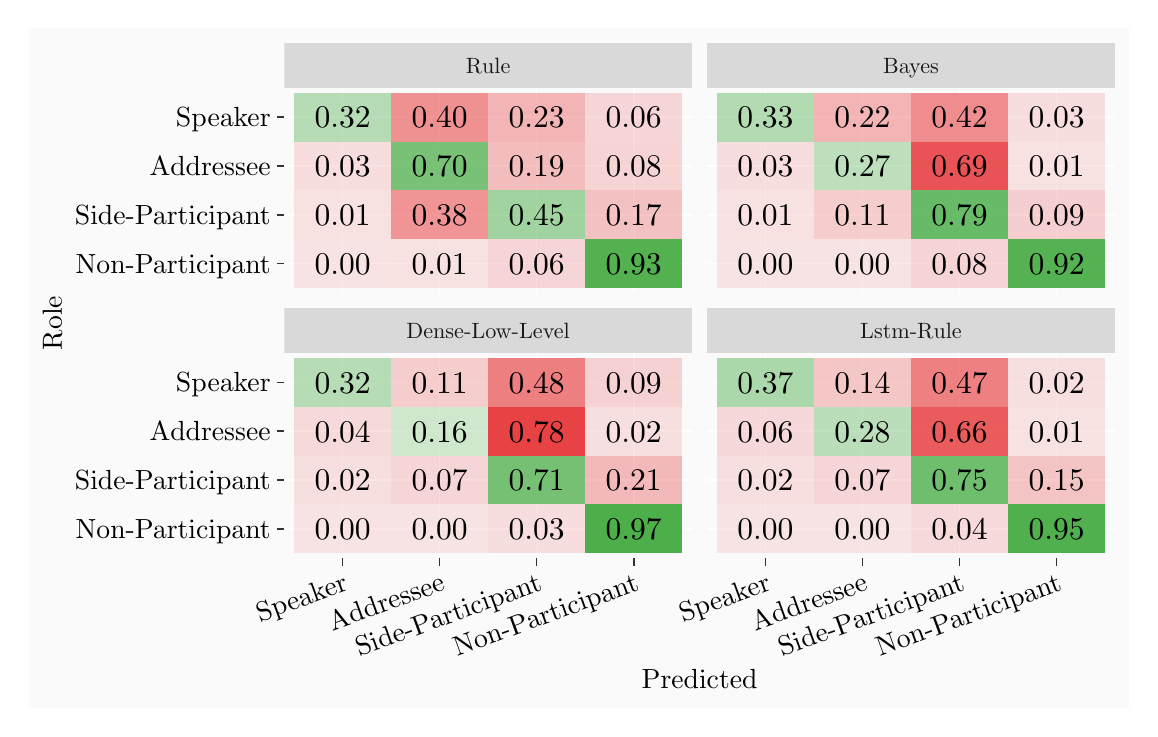
\begin{tikzpicture}[x=1pt,y=1pt]
\definecolor{fillColor}{RGB}{255,255,255}
\path[use as bounding box,fill=fillColor,fill opacity=0.00] (0,0) rectangle (398.34,246.17);
\begin{scope}
\path[clip] (  0.00,  0.00) rectangle (398.34,246.17);
\definecolor{drawColor}{RGB}{255,255,255}
\definecolor{fillColor}{gray}{0.98}

\path[draw=drawColor,line width= 0.6pt,line join=round,line cap=round,fill=fillColor] (  0.00,  0.00) rectangle (398.34,246.17);
\end{scope}
\begin{scope}
\path[clip] ( 92.74,150.34) rectangle (240.04,224.42);
\definecolor{drawColor}{RGB}{255,255,255}

\path[draw=drawColor,line width= 0.6pt,line join=round] ( 92.74,160.93) --
	(240.04,160.93);

\path[draw=drawColor,line width= 0.6pt,line join=round] ( 92.74,178.56) --
	(240.04,178.56);

\path[draw=drawColor,line width= 0.6pt,line join=round] ( 92.74,196.20) --
	(240.04,196.20);

\path[draw=drawColor,line width= 0.6pt,line join=round] ( 92.74,213.84) --
	(240.04,213.84);

\path[draw=drawColor,line width= 0.6pt,line join=round] (113.78,150.34) --
	(113.78,224.42);

\path[draw=drawColor,line width= 0.6pt,line join=round] (148.85,150.34) --
	(148.85,224.42);

\path[draw=drawColor,line width= 0.6pt,line join=round] (183.92,150.34) --
	(183.92,224.42);

\path[draw=drawColor,line width= 0.6pt,line join=round] (218.99,150.34) --
	(218.99,224.42);
\definecolor{fillColor}{RGB}{77,175,74}

\path[fill=fillColor,fill opacity=0.39] ( 96.24,205.02) rectangle (131.32,222.66);
\definecolor{fillColor}{RGB}{228,26,28}

\path[fill=fillColor,fill opacity=0.47] (131.32,205.02) rectangle (166.39,222.66);
\definecolor{fillColor}{RGB}{228,26,28}

\path[fill=fillColor,fill opacity=0.31] (166.39,205.02) rectangle (201.46,222.66);
\definecolor{fillColor}{RGB}{228,26,28}

\path[fill=fillColor,fill opacity=0.16] (201.46,205.02) rectangle (236.53,222.66);
\definecolor{fillColor}{RGB}{228,26,28}

\path[fill=fillColor,fill opacity=0.13] ( 96.24,187.38) rectangle (131.32,205.02);
\definecolor{fillColor}{RGB}{77,175,74}

\path[fill=fillColor,fill opacity=0.75] (131.32,187.38) rectangle (166.39,205.02);
\definecolor{fillColor}{RGB}{228,26,28}

\path[fill=fillColor,fill opacity=0.27] (166.39,187.38) rectangle (201.46,205.02);
\definecolor{fillColor}{RGB}{228,26,28}

\path[fill=fillColor,fill opacity=0.17] (201.46,187.38) rectangle (236.53,205.02);
\definecolor{fillColor}{RGB}{228,26,28}

\path[fill=fillColor,fill opacity=0.11] ( 96.24,169.74) rectangle (131.32,187.38);
\definecolor{fillColor}{RGB}{228,26,28}

\path[fill=fillColor,fill opacity=0.45] (131.32,169.74) rectangle (166.39,187.38);
\definecolor{fillColor}{RGB}{77,175,74}

\path[fill=fillColor,fill opacity=0.51] (166.39,169.74) rectangle (201.46,187.38);
\definecolor{fillColor}{RGB}{228,26,28}

\path[fill=fillColor,fill opacity=0.25] (201.46,169.74) rectangle (236.53,187.38);
\definecolor{fillColor}{RGB}{228,26,28}

\path[fill=fillColor,fill opacity=0.10] ( 96.24,152.11) rectangle (131.32,169.74);
\definecolor{fillColor}{RGB}{228,26,28}

\path[fill=fillColor,fill opacity=0.11] (131.32,152.11) rectangle (166.39,169.74);
\definecolor{fillColor}{RGB}{228,26,28}

\path[fill=fillColor,fill opacity=0.16] (166.39,152.11) rectangle (201.46,169.74);
\definecolor{fillColor}{RGB}{77,175,74}

\path[fill=fillColor,fill opacity=0.96] (201.46,152.11) rectangle (236.53,169.74);
\definecolor{drawColor}{RGB}{0,0,0}

\node[text=drawColor,anchor=base,inner sep=0pt, outer sep=0pt, scale=  1.14] at (113.78,209.92) {0.32};

\node[text=drawColor,anchor=base,inner sep=0pt, outer sep=0pt, scale=  1.14] at (148.85,209.92) {0.40};

\node[text=drawColor,anchor=base,inner sep=0pt, outer sep=0pt, scale=  1.14] at (183.92,209.92) {0.23};

\node[text=drawColor,anchor=base,inner sep=0pt, outer sep=0pt, scale=  1.14] at (218.99,209.92) {0.06};

\node[text=drawColor,anchor=base,inner sep=0pt, outer sep=0pt, scale=  1.14] at (113.78,192.28) {0.03};

\node[text=drawColor,anchor=base,inner sep=0pt, outer sep=0pt, scale=  1.14] at (148.85,192.28) {0.70};

\node[text=drawColor,anchor=base,inner sep=0pt, outer sep=0pt, scale=  1.14] at (183.92,192.28) {0.19};

\node[text=drawColor,anchor=base,inner sep=0pt, outer sep=0pt, scale=  1.14] at (218.99,192.28) {0.08};

\node[text=drawColor,anchor=base,inner sep=0pt, outer sep=0pt, scale=  1.14] at (113.78,174.64) {0.01};

\node[text=drawColor,anchor=base,inner sep=0pt, outer sep=0pt, scale=  1.14] at (148.85,174.64) {0.38};

\node[text=drawColor,anchor=base,inner sep=0pt, outer sep=0pt, scale=  1.14] at (183.92,174.64) {0.45};

\node[text=drawColor,anchor=base,inner sep=0pt, outer sep=0pt, scale=  1.14] at (218.99,174.64) {0.17};

\node[text=drawColor,anchor=base,inner sep=0pt, outer sep=0pt, scale=  1.14] at (113.78,157.01) {0.00};

\node[text=drawColor,anchor=base,inner sep=0pt, outer sep=0pt, scale=  1.14] at (148.85,157.01) {0.01};

\node[text=drawColor,anchor=base,inner sep=0pt, outer sep=0pt, scale=  1.14] at (183.92,157.01) {0.06};

\node[text=drawColor,anchor=base,inner sep=0pt, outer sep=0pt, scale=  1.14] at (218.99,157.01) {0.93};
\end{scope}
\begin{scope}
\path[clip] ( 92.74, 54.51) rectangle (240.04,128.59);
\definecolor{drawColor}{RGB}{255,255,255}

\path[draw=drawColor,line width= 0.6pt,line join=round] ( 92.74, 65.09) --
	(240.04, 65.09);

\path[draw=drawColor,line width= 0.6pt,line join=round] ( 92.74, 82.73) --
	(240.04, 82.73);

\path[draw=drawColor,line width= 0.6pt,line join=round] ( 92.74,100.37) --
	(240.04,100.37);

\path[draw=drawColor,line width= 0.6pt,line join=round] ( 92.74,118.01) --
	(240.04,118.01);

\path[draw=drawColor,line width= 0.6pt,line join=round] (113.78, 54.51) --
	(113.78,128.59);

\path[draw=drawColor,line width= 0.6pt,line join=round] (148.85, 54.51) --
	(148.85,128.59);

\path[draw=drawColor,line width= 0.6pt,line join=round] (183.92, 54.51) --
	(183.92,128.59);

\path[draw=drawColor,line width= 0.6pt,line join=round] (218.99, 54.51) --
	(218.99,128.59);
\definecolor{fillColor}{RGB}{77,175,74}

\path[fill=fillColor,fill opacity=0.39] ( 96.24,109.19) rectangle (131.32,126.83);
\definecolor{fillColor}{RGB}{228,26,28}

\path[fill=fillColor,fill opacity=0.20] (131.32,109.19) rectangle (166.39,126.83);
\definecolor{fillColor}{RGB}{228,26,28}

\path[fill=fillColor,fill opacity=0.55] (166.39,109.19) rectangle (201.46,126.83);
\definecolor{fillColor}{RGB}{228,26,28}

\path[fill=fillColor,fill opacity=0.18] (201.46,109.19) rectangle (236.53,126.83);
\definecolor{fillColor}{RGB}{228,26,28}

\path[fill=fillColor,fill opacity=0.14] ( 96.24, 91.55) rectangle (131.32,109.19);
\definecolor{fillColor}{RGB}{77,175,74}

\path[fill=fillColor,fill opacity=0.25] (131.32, 91.55) rectangle (166.39,109.19);
\definecolor{fillColor}{RGB}{228,26,28}

\path[fill=fillColor,fill opacity=0.82] (166.39, 91.55) rectangle (201.46,109.19);
\definecolor{fillColor}{RGB}{228,26,28}

\path[fill=fillColor,fill opacity=0.12] (201.46, 91.55) rectangle (236.53,109.19);
\definecolor{fillColor}{RGB}{228,26,28}

\path[fill=fillColor,fill opacity=0.12] ( 96.24, 73.91) rectangle (131.32, 91.55);
\definecolor{fillColor}{RGB}{228,26,28}

\path[fill=fillColor,fill opacity=0.16] (131.32, 73.91) rectangle (166.39, 91.55);
\definecolor{fillColor}{RGB}{77,175,74}

\path[fill=fillColor,fill opacity=0.76] (166.39, 73.91) rectangle (201.46, 91.55);
\definecolor{fillColor}{RGB}{228,26,28}

\path[fill=fillColor,fill opacity=0.29] (201.46, 73.91) rectangle (236.53, 91.55);
\definecolor{fillColor}{RGB}{228,26,28}

\path[fill=fillColor,fill opacity=0.10] ( 96.24, 56.28) rectangle (131.32, 73.91);

\path[fill=fillColor,fill opacity=0.10] (131.32, 56.28) rectangle (166.39, 73.91);
\definecolor{fillColor}{RGB}{228,26,28}

\path[fill=fillColor,fill opacity=0.13] (166.39, 56.28) rectangle (201.46, 73.91);
\definecolor{fillColor}{RGB}{77,175,74}

\path[fill=fillColor] (201.46, 56.28) rectangle (236.53, 73.91);
\definecolor{drawColor}{RGB}{0,0,0}

\node[text=drawColor,anchor=base,inner sep=0pt, outer sep=0pt, scale=  1.14] at (113.78,114.09) {0.32};

\node[text=drawColor,anchor=base,inner sep=0pt, outer sep=0pt, scale=  1.14] at (148.85,114.09) {0.11};

\node[text=drawColor,anchor=base,inner sep=0pt, outer sep=0pt, scale=  1.14] at (183.92,114.09) {0.48};

\node[text=drawColor,anchor=base,inner sep=0pt, outer sep=0pt, scale=  1.14] at (218.99,114.09) {0.09};

\node[text=drawColor,anchor=base,inner sep=0pt, outer sep=0pt, scale=  1.14] at (113.78, 96.45) {0.04};

\node[text=drawColor,anchor=base,inner sep=0pt, outer sep=0pt, scale=  1.14] at (148.85, 96.45) {0.16};

\node[text=drawColor,anchor=base,inner sep=0pt, outer sep=0pt, scale=  1.14] at (183.92, 96.45) {0.78};

\node[text=drawColor,anchor=base,inner sep=0pt, outer sep=0pt, scale=  1.14] at (218.99, 96.45) {0.02};

\node[text=drawColor,anchor=base,inner sep=0pt, outer sep=0pt, scale=  1.14] at (113.78, 78.81) {0.02};

\node[text=drawColor,anchor=base,inner sep=0pt, outer sep=0pt, scale=  1.14] at (148.85, 78.81) {0.07};

\node[text=drawColor,anchor=base,inner sep=0pt, outer sep=0pt, scale=  1.14] at (183.92, 78.81) {0.71};

\node[text=drawColor,anchor=base,inner sep=0pt, outer sep=0pt, scale=  1.14] at (218.99, 78.81) {0.21};

\node[text=drawColor,anchor=base,inner sep=0pt, outer sep=0pt, scale=  1.14] at (113.78, 61.18) {0.00};

\node[text=drawColor,anchor=base,inner sep=0pt, outer sep=0pt, scale=  1.14] at (148.85, 61.18) {0.00};

\node[text=drawColor,anchor=base,inner sep=0pt, outer sep=0pt, scale=  1.14] at (183.92, 61.18) {0.03};

\node[text=drawColor,anchor=base,inner sep=0pt, outer sep=0pt, scale=  1.14] at (218.99, 61.18) {0.97};
\end{scope}
\begin{scope}
\path[clip] (245.54,150.34) rectangle (392.84,224.42);
\definecolor{drawColor}{RGB}{255,255,255}

\path[draw=drawColor,line width= 0.6pt,line join=round] (245.54,160.93) --
	(392.84,160.93);

\path[draw=drawColor,line width= 0.6pt,line join=round] (245.54,178.56) --
	(392.84,178.56);

\path[draw=drawColor,line width= 0.6pt,line join=round] (245.54,196.20) --
	(392.84,196.20);

\path[draw=drawColor,line width= 0.6pt,line join=round] (245.54,213.84) --
	(392.84,213.84);

\path[draw=drawColor,line width= 0.6pt,line join=round] (266.58,150.34) --
	(266.58,224.42);

\path[draw=drawColor,line width= 0.6pt,line join=round] (301.65,150.34) --
	(301.65,224.42);

\path[draw=drawColor,line width= 0.6pt,line join=round] (336.72,150.34) --
	(336.72,224.42);

\path[draw=drawColor,line width= 0.6pt,line join=round] (371.80,150.34) --
	(371.80,224.42);
\definecolor{fillColor}{RGB}{77,175,74}

\path[fill=fillColor,fill opacity=0.41] (249.04,205.02) rectangle (284.12,222.66);
\definecolor{fillColor}{RGB}{228,26,28}

\path[fill=fillColor,fill opacity=0.31] (284.12,205.02) rectangle (319.19,222.66);
\definecolor{fillColor}{RGB}{228,26,28}

\path[fill=fillColor,fill opacity=0.49] (319.19,205.02) rectangle (354.26,222.66);
\definecolor{fillColor}{RGB}{228,26,28}

\path[fill=fillColor,fill opacity=0.13] (354.26,205.02) rectangle (389.33,222.66);
\definecolor{fillColor}{RGB}{228,26,28}

\path[fill=fillColor,fill opacity=0.13] (249.04,187.38) rectangle (284.12,205.02);
\definecolor{fillColor}{RGB}{77,175,74}

\path[fill=fillColor,fill opacity=0.35] (284.12,187.38) rectangle (319.19,205.02);
\definecolor{fillColor}{RGB}{228,26,28}

\path[fill=fillColor,fill opacity=0.74] (319.19,187.38) rectangle (354.26,205.02);
\definecolor{fillColor}{RGB}{228,26,28}

\path[fill=fillColor,fill opacity=0.11] (354.26,187.38) rectangle (389.33,205.02);
\definecolor{fillColor}{RGB}{228,26,28}

\path[fill=fillColor,fill opacity=0.11] (249.04,169.74) rectangle (284.12,187.38);
\definecolor{fillColor}{RGB}{228,26,28}

\path[fill=fillColor,fill opacity=0.20] (284.12,169.74) rectangle (319.19,187.38);
\definecolor{fillColor}{RGB}{77,175,74}

\path[fill=fillColor,fill opacity=0.84] (319.19,169.74) rectangle (354.26,187.38);
\definecolor{fillColor}{RGB}{228,26,28}

\path[fill=fillColor,fill opacity=0.19] (354.26,169.74) rectangle (389.33,187.38);
\definecolor{fillColor}{RGB}{228,26,28}

\path[fill=fillColor,fill opacity=0.10] (249.04,152.11) rectangle (284.12,169.74);

\path[fill=fillColor,fill opacity=0.10] (284.12,152.11) rectangle (319.19,169.74);
\definecolor{fillColor}{RGB}{228,26,28}

\path[fill=fillColor,fill opacity=0.17] (319.19,152.11) rectangle (354.26,169.74);
\definecolor{fillColor}{RGB}{77,175,74}

\path[fill=fillColor,fill opacity=0.95] (354.26,152.11) rectangle (389.33,169.74);
\definecolor{drawColor}{RGB}{0,0,0}

\node[text=drawColor,anchor=base,inner sep=0pt, outer sep=0pt, scale=  1.14] at (266.58,209.92) {0.33};

\node[text=drawColor,anchor=base,inner sep=0pt, outer sep=0pt, scale=  1.14] at (301.65,209.92) {0.22};

\node[text=drawColor,anchor=base,inner sep=0pt, outer sep=0pt, scale=  1.14] at (336.72,209.92) {0.42};

\node[text=drawColor,anchor=base,inner sep=0pt, outer sep=0pt, scale=  1.14] at (371.80,209.92) {0.03};

\node[text=drawColor,anchor=base,inner sep=0pt, outer sep=0pt, scale=  1.14] at (266.58,192.28) {0.03};

\node[text=drawColor,anchor=base,inner sep=0pt, outer sep=0pt, scale=  1.14] at (301.65,192.28) {0.27};

\node[text=drawColor,anchor=base,inner sep=0pt, outer sep=0pt, scale=  1.14] at (336.72,192.28) {0.69};

\node[text=drawColor,anchor=base,inner sep=0pt, outer sep=0pt, scale=  1.14] at (371.80,192.28) {0.01};

\node[text=drawColor,anchor=base,inner sep=0pt, outer sep=0pt, scale=  1.14] at (266.58,174.64) {0.01};

\node[text=drawColor,anchor=base,inner sep=0pt, outer sep=0pt, scale=  1.14] at (301.65,174.64) {0.11};

\node[text=drawColor,anchor=base,inner sep=0pt, outer sep=0pt, scale=  1.14] at (336.72,174.64) {0.79};

\node[text=drawColor,anchor=base,inner sep=0pt, outer sep=0pt, scale=  1.14] at (371.80,174.64) {0.09};

\node[text=drawColor,anchor=base,inner sep=0pt, outer sep=0pt, scale=  1.14] at (266.58,157.01) {0.00};

\node[text=drawColor,anchor=base,inner sep=0pt, outer sep=0pt, scale=  1.14] at (301.65,157.01) {0.00};

\node[text=drawColor,anchor=base,inner sep=0pt, outer sep=0pt, scale=  1.14] at (336.72,157.01) {0.08};

\node[text=drawColor,anchor=base,inner sep=0pt, outer sep=0pt, scale=  1.14] at (371.80,157.01) {0.92};
\end{scope}
\begin{scope}
\path[clip] (245.54, 54.51) rectangle (392.84,128.59);
\definecolor{drawColor}{RGB}{255,255,255}

\path[draw=drawColor,line width= 0.6pt,line join=round] (245.54, 65.09) --
	(392.84, 65.09);

\path[draw=drawColor,line width= 0.6pt,line join=round] (245.54, 82.73) --
	(392.84, 82.73);

\path[draw=drawColor,line width= 0.6pt,line join=round] (245.54,100.37) --
	(392.84,100.37);

\path[draw=drawColor,line width= 0.6pt,line join=round] (245.54,118.01) --
	(392.84,118.01);

\path[draw=drawColor,line width= 0.6pt,line join=round] (266.58, 54.51) --
	(266.58,128.59);

\path[draw=drawColor,line width= 0.6pt,line join=round] (301.65, 54.51) --
	(301.65,128.59);

\path[draw=drawColor,line width= 0.6pt,line join=round] (336.72, 54.51) --
	(336.72,128.59);

\path[draw=drawColor,line width= 0.6pt,line join=round] (371.80, 54.51) --
	(371.80,128.59);
\definecolor{fillColor}{RGB}{77,175,74}

\path[fill=fillColor,fill opacity=0.45] (249.04,109.19) rectangle (284.12,126.83);
\definecolor{fillColor}{RGB}{228,26,28}

\path[fill=fillColor,fill opacity=0.23] (284.12,109.19) rectangle (319.19,126.83);
\definecolor{fillColor}{RGB}{228,26,28}

\path[fill=fillColor,fill opacity=0.54] (319.19,109.19) rectangle (354.26,126.83);
\definecolor{fillColor}{RGB}{228,26,28}

\path[fill=fillColor,fill opacity=0.12] (354.26,109.19) rectangle (389.33,126.83);
\definecolor{fillColor}{RGB}{228,26,28}

\path[fill=fillColor,fill opacity=0.15] (249.04, 91.55) rectangle (284.12,109.19);
\definecolor{fillColor}{RGB}{77,175,74}

\path[fill=fillColor,fill opacity=0.36] (284.12, 91.55) rectangle (319.19,109.19);
\definecolor{fillColor}{RGB}{228,26,28}

\path[fill=fillColor,fill opacity=0.71] (319.19, 91.55) rectangle (354.26,109.19);
\definecolor{fillColor}{RGB}{228,26,28}

\path[fill=fillColor,fill opacity=0.11] (354.26, 91.55) rectangle (389.33,109.19);
\definecolor{fillColor}{RGB}{228,26,28}

\path[fill=fillColor,fill opacity=0.12] (249.04, 73.91) rectangle (284.12, 91.55);
\definecolor{fillColor}{RGB}{228,26,28}

\path[fill=fillColor,fill opacity=0.16] (284.12, 73.91) rectangle (319.19, 91.55);
\definecolor{fillColor}{RGB}{77,175,74}

\path[fill=fillColor,fill opacity=0.80] (319.19, 73.91) rectangle (354.26, 91.55);
\definecolor{fillColor}{RGB}{228,26,28}

\path[fill=fillColor,fill opacity=0.24] (354.26, 73.91) rectangle (389.33, 91.55);
\definecolor{fillColor}{RGB}{228,26,28}

\path[fill=fillColor,fill opacity=0.10] (249.04, 56.28) rectangle (284.12, 73.91);

\path[fill=fillColor,fill opacity=0.10] (284.12, 56.28) rectangle (319.19, 73.91);
\definecolor{fillColor}{RGB}{228,26,28}

\path[fill=fillColor,fill opacity=0.14] (319.19, 56.28) rectangle (354.26, 73.91);
\definecolor{fillColor}{RGB}{77,175,74}

\path[fill=fillColor,fill opacity=0.98] (354.26, 56.28) rectangle (389.33, 73.91);
\definecolor{drawColor}{RGB}{0,0,0}

\node[text=drawColor,anchor=base,inner sep=0pt, outer sep=0pt, scale=  1.14] at (266.58,114.09) {0.37};

\node[text=drawColor,anchor=base,inner sep=0pt, outer sep=0pt, scale=  1.14] at (301.65,114.09) {0.14};

\node[text=drawColor,anchor=base,inner sep=0pt, outer sep=0pt, scale=  1.14] at (336.72,114.09) {0.47};

\node[text=drawColor,anchor=base,inner sep=0pt, outer sep=0pt, scale=  1.14] at (371.80,114.09) {0.02};

\node[text=drawColor,anchor=base,inner sep=0pt, outer sep=0pt, scale=  1.14] at (266.58, 96.45) {0.06};

\node[text=drawColor,anchor=base,inner sep=0pt, outer sep=0pt, scale=  1.14] at (301.65, 96.45) {0.28};

\node[text=drawColor,anchor=base,inner sep=0pt, outer sep=0pt, scale=  1.14] at (336.72, 96.45) {0.66};

\node[text=drawColor,anchor=base,inner sep=0pt, outer sep=0pt, scale=  1.14] at (371.80, 96.45) {0.01};

\node[text=drawColor,anchor=base,inner sep=0pt, outer sep=0pt, scale=  1.14] at (266.58, 78.81) {0.02};

\node[text=drawColor,anchor=base,inner sep=0pt, outer sep=0pt, scale=  1.14] at (301.65, 78.81) {0.07};

\node[text=drawColor,anchor=base,inner sep=0pt, outer sep=0pt, scale=  1.14] at (336.72, 78.81) {0.75};

\node[text=drawColor,anchor=base,inner sep=0pt, outer sep=0pt, scale=  1.14] at (371.80, 78.81) {0.15};

\node[text=drawColor,anchor=base,inner sep=0pt, outer sep=0pt, scale=  1.14] at (266.58, 61.18) {0.00};

\node[text=drawColor,anchor=base,inner sep=0pt, outer sep=0pt, scale=  1.14] at (301.65, 61.18) {0.00};

\node[text=drawColor,anchor=base,inner sep=0pt, outer sep=0pt, scale=  1.14] at (336.72, 61.18) {0.04};

\node[text=drawColor,anchor=base,inner sep=0pt, outer sep=0pt, scale=  1.14] at (371.80, 61.18) {0.95};
\end{scope}
\begin{scope}
\path[clip] ( 92.74,128.59) rectangle (240.04,144.84);
\definecolor{fillColor}{gray}{0.85}

\path[fill=fillColor] ( 92.74,128.59) rectangle (240.04,144.84);
\definecolor{drawColor}{gray}{0.10}

\node[text=drawColor,anchor=base,inner sep=0pt, outer sep=0pt, scale=  0.80] at (166.39,133.96) {Dense-Low-Level};
\end{scope}
\begin{scope}
\path[clip] (245.54,128.59) rectangle (392.84,144.84);
\definecolor{fillColor}{gray}{0.85}

\path[fill=fillColor] (245.54,128.59) rectangle (392.84,144.84);
\definecolor{drawColor}{gray}{0.10}

\node[text=drawColor,anchor=base,inner sep=0pt, outer sep=0pt, scale=  0.80] at (319.19,133.96) {Lstm-Rule};
\end{scope}
\begin{scope}
\path[clip] ( 92.74,224.42) rectangle (240.04,240.67);
\definecolor{fillColor}{gray}{0.85}

\path[fill=fillColor] ( 92.74,224.42) rectangle (240.04,240.67);
\definecolor{drawColor}{gray}{0.10}

\node[text=drawColor,anchor=base,inner sep=0pt, outer sep=0pt, scale=  0.80] at (166.39,229.79) {Rule};
\end{scope}
\begin{scope}
\path[clip] (245.54,224.42) rectangle (392.84,240.67);
\definecolor{fillColor}{gray}{0.85}

\path[fill=fillColor] (245.54,224.42) rectangle (392.84,240.67);
\definecolor{drawColor}{gray}{0.10}

\node[text=drawColor,anchor=base,inner sep=0pt, outer sep=0pt, scale=  0.80] at (319.19,229.79) {Bayes};
\end{scope}
\begin{scope}
\path[clip] (  0.00,  0.00) rectangle (398.34,246.17);
\definecolor{drawColor}{gray}{0.20}

\path[draw=drawColor,line width= 0.6pt,line join=round] (113.78, 51.76) --
	(113.78, 54.51);

\path[draw=drawColor,line width= 0.6pt,line join=round] (148.85, 51.76) --
	(148.85, 54.51);

\path[draw=drawColor,line width= 0.6pt,line join=round] (183.92, 51.76) --
	(183.92, 54.51);

\path[draw=drawColor,line width= 0.6pt,line join=round] (218.99, 51.76) --
	(218.99, 54.51);
\end{scope}
\begin{scope}
\path[clip] (  0.00,  0.00) rectangle (398.34,246.17);
\definecolor{drawColor}{RGB}{0,0,0}

\node[text=drawColor,rotate= 20.00,anchor=base east,inner sep=0pt, outer sep=0pt, scale=  1.00] at (116.13, 43.09) {Speaker};

\node[text=drawColor,rotate= 20.00,anchor=base east,inner sep=0pt, outer sep=0pt, scale=  1.00] at (151.21, 43.09) {Addressee};

\node[text=drawColor,rotate= 20.00,anchor=base east,inner sep=0pt, outer sep=0pt, scale=  1.00] at (186.28, 43.09) {Side-Participant};

\node[text=drawColor,rotate= 20.00,anchor=base east,inner sep=0pt, outer sep=0pt, scale=  1.00] at (221.35, 43.09) {Non-Participant};
\end{scope}
\begin{scope}
\path[clip] (  0.00,  0.00) rectangle (398.34,246.17);
\definecolor{drawColor}{gray}{0.20}

\path[draw=drawColor,line width= 0.6pt,line join=round] (266.58, 51.76) --
	(266.58, 54.51);

\path[draw=drawColor,line width= 0.6pt,line join=round] (301.65, 51.76) --
	(301.65, 54.51);

\path[draw=drawColor,line width= 0.6pt,line join=round] (336.72, 51.76) --
	(336.72, 54.51);

\path[draw=drawColor,line width= 0.6pt,line join=round] (371.80, 51.76) --
	(371.80, 54.51);
\end{scope}
\begin{scope}
\path[clip] (  0.00,  0.00) rectangle (398.34,246.17);
\definecolor{drawColor}{RGB}{0,0,0}

\node[text=drawColor,rotate= 20.00,anchor=base east,inner sep=0pt, outer sep=0pt, scale=  1.00] at (268.94, 43.09) {Speaker};

\node[text=drawColor,rotate= 20.00,anchor=base east,inner sep=0pt, outer sep=0pt, scale=  1.00] at (304.01, 43.09) {Addressee};

\node[text=drawColor,rotate= 20.00,anchor=base east,inner sep=0pt, outer sep=0pt, scale=  1.00] at (339.08, 43.09) {Side-Participant};

\node[text=drawColor,rotate= 20.00,anchor=base east,inner sep=0pt, outer sep=0pt, scale=  1.00] at (374.15, 43.09) {Non-Participant};
\end{scope}
\begin{scope}
\path[clip] (  0.00,  0.00) rectangle (398.34,246.17);
\definecolor{drawColor}{RGB}{0,0,0}

\node[text=drawColor,anchor=base east,inner sep=0pt, outer sep=0pt, scale=  1.00] at ( 87.79,157.48) {Non-Participant};

\node[text=drawColor,anchor=base east,inner sep=0pt, outer sep=0pt, scale=  1.00] at ( 87.79,175.12) {Side-Participant};

\node[text=drawColor,anchor=base east,inner sep=0pt, outer sep=0pt, scale=  1.00] at ( 87.79,192.76) {Addressee};

\node[text=drawColor,anchor=base east,inner sep=0pt, outer sep=0pt, scale=  1.00] at ( 87.79,210.39) {Speaker};
\end{scope}
\begin{scope}
\path[clip] (  0.00,  0.00) rectangle (398.34,246.17);
\definecolor{drawColor}{gray}{0.20}

\path[draw=drawColor,line width= 0.6pt,line join=round] ( 89.99,160.93) --
	( 92.74,160.93);

\path[draw=drawColor,line width= 0.6pt,line join=round] ( 89.99,178.56) --
	( 92.74,178.56);

\path[draw=drawColor,line width= 0.6pt,line join=round] ( 89.99,196.20) --
	( 92.74,196.20);

\path[draw=drawColor,line width= 0.6pt,line join=round] ( 89.99,213.84) --
	( 92.74,213.84);
\end{scope}
\begin{scope}
\path[clip] (  0.00,  0.00) rectangle (398.34,246.17);
\definecolor{drawColor}{RGB}{0,0,0}

\node[text=drawColor,anchor=base east,inner sep=0pt, outer sep=0pt, scale=  1.00] at ( 87.79, 61.65) {Non-Participant};

\node[text=drawColor,anchor=base east,inner sep=0pt, outer sep=0pt, scale=  1.00] at ( 87.79, 79.29) {Side-Participant};

\node[text=drawColor,anchor=base east,inner sep=0pt, outer sep=0pt, scale=  1.00] at ( 87.79, 96.93) {Addressee};

\node[text=drawColor,anchor=base east,inner sep=0pt, outer sep=0pt, scale=  1.00] at ( 87.79,114.56) {Speaker};
\end{scope}
\begin{scope}
\path[clip] (  0.00,  0.00) rectangle (398.34,246.17);
\definecolor{drawColor}{gray}{0.20}

\path[draw=drawColor,line width= 0.6pt,line join=round] ( 89.99, 65.09) --
	( 92.74, 65.09);

\path[draw=drawColor,line width= 0.6pt,line join=round] ( 89.99, 82.73) --
	( 92.74, 82.73);

\path[draw=drawColor,line width= 0.6pt,line join=round] ( 89.99,100.37) --
	( 92.74,100.37);

\path[draw=drawColor,line width= 0.6pt,line join=round] ( 89.99,118.01) --
	( 92.74,118.01);
\end{scope}
\begin{scope}
\path[clip] (  0.00,  0.00) rectangle (398.34,246.17);
\definecolor{drawColor}{RGB}{0,0,0}

\node[text=drawColor,anchor=base,inner sep=0pt, outer sep=0pt, scale=  1.00] at (242.79,  7.44) {Predicted};
\end{scope}
\begin{scope}
\path[clip] (  0.00,  0.00) rectangle (398.34,246.17);
\definecolor{drawColor}{RGB}{0,0,0}

\node[text=drawColor,rotate= 90.00,anchor=base,inner sep=0pt, outer sep=0pt, scale=  1.00] at ( 12.39,139.47) {Role};
\end{scope}
\end{tikzpicture}
